Comme il a été présenté dans l'introduction sur l'intelligence artificielle, et vu en pratique dans la structure de base d'un comportement Lua interprétable par ARGoS, un footbot exécute à chaque step une séquence d'opérations. On peut distinguer dans cette séquence trois types d'opérations (cf chapitre \ref{chap:AI}): l'écoute des capteurs, la prise de décision et les interactions sur l'environnement par l'intermédiaire des effecteurs, que l'on nommera ici simplement sous le nom d'actions. Ces actions sont donc limitées et déterminées par les effecteurs dont dispose le robot et qui sont décrits au chapitre \ref{chap:argosFootbot}. Dans ce chapitre-ci, l'un des effecteurs primordiaux d'un footbot sera examiné: son déplacement.

\section{Aspects physiques du déplacement}

Tout d'abord, il est intéressant de se pencher sur le lien entre les paramètres physiques du robot et la manière dont celui-ci peut effectuer l'action simple «se rendre d'un point A à un point B» dans le cas où le robot agit seul dans un environnement sans obstacles. Ensuite, nous verrons comment le robot peut s’accommoder des obstacles (fixes, prévisibles) et autres robots (mobiles, imprévisibles) à partir d'une ou plusieurs de ces actions simples.

\begin{wrapfigure}{r}{0.3\textwidth}
  \vspace{-3em}
  \begin{center}
    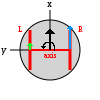
\includegraphics[width=0.15\textwidth]{pics/robotWheels.png}
  \end{center}
  \vspace{-2em}
  \caption{Signification physique de \(v_r,\: v_l,\: v_g \; et \; \omega_g \) \cite{argosSite1}}
  \vspace{-1em}
  \end{wrapfigure}
L'effecteur dont un footbot dispose afin de se déplacer est une paire de roues dont les vitesses peuvent être fixées de manière indépendante. A chaque instant, les seuls deux mouvements auxquels peut accéder le robot sont donc une translation parallèle aux roues et une rotation autour d'un point au milieu de l'axe des roues. La mécanique~\cite{meca} nous indique que la composition de ces deux mouvements est suffisante pour permettre au robot de se déplacer librement dans un plan mais surtout, elle nous donne la relation entre les vitesses des deux roues et la vitesse générale ainsi que la vitesse de rotation du robot:
\begin{equation}
\begin{cases}
v_g=\frac{v_r+v_l}{2}\\
\omega_g=\frac{v_r-v_l}{l_{axe}}
\end{cases}  
\end{equation}

\section{Déplacement sans obstacles}

A partir de cette loi des vitesses, il est aisé de construire un algorithme permettant à un robot de converger vers sont but selon une trajectoire souple et à vitesse constante.

\begin{algorithm}                    
\caption{Convergence with no obstacle avoidance}
\label{simpleConvergence}
\begin{algorithmic}
  \REQUIRE \(SPEED \equiv \) Fixed speed of the footbot \(> 0\)
  \REQUIRE Goal in arena
  \ENSURE footbot converges towards the goal at speed \(SPEED\)
  \WHILE{goal not reached}
    \STATE update footbot position and orientation
    \STATE calculate \( \theta \equiv\) angle between the direction of the goal from the footbot and footbot orientation
    \STATE \( right\:velocity \gets\) convergence(\(\theta,\:SPEED\))
    \STATE \( left\:velocity \gets 2 \times SPEED-right\:velocity\) \COMMENT{so that overall speed stays equal to SPEED}
  \ENDWHILE
\end{algorithmic}
\end{algorithm}

Où convergence($\theta, SPEED$) fixe la convergence du robot vers son goal. Elle doit satisfaire:

\begin{equation}
  \begin{cases}
    convergence(0,SPEED)=SPEED\\
    convergence(\overset{\text{goal à gauche du robot}}{\overbrace{0<\theta\leq\pi}},SPEED)>SPEED\\
    convergence(\overset{\text{goal à droite du robot}}{\overbrace{0>\theta\geq-\pi}},SPEED)<SPEED
  \end{cases}
\end{equation}

Pour une fonction convergence($\theta, SPEED$) donnée satisfaisant à cette condition (par exemple dépendance linéaire en \(\theta\)), le footbot peut donc se rendre d'un point A à un point B, tant qu'il ne rencontre pas d'obstacles sur son trajet. Notons que cet algorithme s'intègre particulièrement bien dans la fonction \emph{step} demandée par ARGoS. Dans notre projet nous avons choisi
\[
convergence(\theta, SPEED)=
\begin{cases}
      { \left( \frac{\pi- \lvert \theta \rvert }{\pi} \right)}^{\kappa} \times SPEED & \text{si } \theta \geq 0\\
      \left( 2 - { \left( \frac{\pi- \lvert \theta \rvert }{\pi} \right) }^{\kappa} \right) \times SPEED & \text{si } \theta < 0
\end{cases}
\]
Où $\kappa > 0$ est un paramètre qui fixe l'intensité de la convergence.

\section{Évitement \emph{greedy} d'obstacles lointains}

Une première manière de permettre au robot d'éviter des obstacles est d'activer le capteur \emph{distance scanner} longue distance qui permet de détecter des obstacles jusqu'à 150cm du footbot. Un évitement très efficace mais parfois trop gourmand consiste alors à chercher à chaque pas la direction la plus proche de la direction du goal et pour laquelle l'obstacle repéré est le plus éloigné du robot (ou non existant) et à converger vers celle-ci. Ceci permet au robot d'éviter plusieurs obstacles à la fois, tout en gardant une trajectoire très optimisée.

\begin{algorithm}                    
\caption{Convergence with greedy obstacle avoidance}
\label{greedyConvergence}
\begin{algorithmic}
  \WHILE{goal not reached}
    \STATE update footbot position and orientation
    \STATE find \( \theta \equiv\) angle between footbot orientation and best direction (closest to goal, least obstacles)
    \STATE \( right\:velocity \gets\) convergence(\(\theta,\:SPEED\))
    \STATE \( left\:velocity \gets 2 \times SPEED-right\:velocity\) \COMMENT{so that overall speed stays equal to SPEED}
  \ENDWHILE
\end{algorithmic}
\end{algorithm}

La fonction convergence doit satisfaire au mêmes contraintes que précédemment et reste inchangée dans notre projet. Pour que l'évitement soit efficace, il faut que $\kappa$ soit assez élevé pour que le footbot s'oriente rapidement vers la direction optimale. Malgré cela, cet évitement reste très \emph{greedy}, dans le sens ou chercher absolument la direction la plus proche de celle du but peut mener à des collisions à cause de différents facteurs et approximations (footbot de taille non nulle, rayons du \emph{distance scanner} parfaitement tangent à un obstacle, \emph{distance scanner} ne faisant pas une mesure par direction à chaque pas, nombre de directions mesurées bien évidemment fini, \ldots). Une première manière de pallier à cela est de regrouper plusieurs mesures voisines en gardant systématiquement la mesure la moins optimiste. Magré cela, un évitement plus sûr d'obstacles proches est aussi nécessaire pour limiter le plus possible les collisions.

Cet évitement d'obstacles est directement utilisé dans notre projet. Son implémentation est détaillée dans l'annexe \ref{app:implEvitGreedy}

\section{Evitement sûr d'obstacles proches\label{sec:emerAvoid}}

La manière la plus directe de permettre au footbot d'éviter des obstacles ou autres robots lorqu'ils sont dangereusement proches est d'alors exécuter une routine d'évitement à la place de la routine de convergence précédente.
\begin{algorithm}
\label{obstacleConvergence}
\caption{Convergence with close obstacle avoidance}
\begin{algorithmic}
  \ENSURE footbot converges towards the goal at speed \(SPEED\) while avoiding obstacles
  \WHILE{goal not reached}
    \STATE update footbot position and orientation
    \STATE read proximity sensors \COMMENT{or whatever other sensor in use}
    \IF{no obstacles too close}
      \STATE do previous convergence
    \ELSE
      \STATE \( right\:velocity \leftarrow\) avoidance(proximity sensor reading, \(SPEED\))
    \ENDIF
    \STATE \( left\:velocity \leftarrow 2 \times SPEED-right\:velocity\) \COMMENT{so that overall speed stays equal to SPEED}
  \ENDWHILE
\end{algorithmic}
\end{algorithm}

Où avoidance(proximity sensor reading, $SPEED$) fixe la routine d'évitement du robot. Son implémentation est très libre et peut fortement varier en fonction du capteur utilisé pour détecter les obstacles. On peut par exemple utiliser le senseur \emph{proximity} du footbot, qui associe à 24 directions autour du robot une valeur entre zéro et un: une valeur zéro indique qu'aucun obstacle n'est perçu à moins de 10cm dans la direction donnée tandis qu'une valeur supérieure indique qu'un objet a été détecté. Cette valeur augmente au fur et à mesure que le robot se rapproche de l'obstacle.~\cite{argosSite1}

Dans notre projet nous avons choisi
\[avoidance(dir, prox)=
  \begin{cases}
      \frac{-\alpha +(1-prox)^{\beta}\cdot dir}{11}SPEED & \text{si }dir \leq 12\\
      \frac{(22+\alpha )-(1-prox)^{\beta}\cdot (25-dir)}{11}SPEED & \text{si }dir \geq 12\\
  \end{cases}
\]

Où $ 1 \leq dir \leq 12 $ est la direction de l'obstacle perçu le plus proche et \hbox{$0 \leq prox \leq 1$} donne la proximité de cette obstacle. Comme présenté plus haut, ce sont les deux informations dont on dispose si l'on utilise le capteur de proximité.  \(1 \leq \alpha \leq 12 \) est un paramètre qui fixe l'influence de la direction de l'obstacle le plus proche et \(0 \leq \beta \) fixe l'influence de la proximité de cette obstacle. Cet évitement est partiellement tiré des exemples fourni sur le site du cours présentant ARGoS \cite{argosSite1}.

\section{Evitement intermédiaire}

Additionnellement, il est possible d'utiliser le capteur \emph{short range} du \emph{distance scanner} pour que le robot puisse déjà commencer à dévier sa trajectoire s'il détecte des obstacles proche de moins de 30cm~\cite{argosSite1}. Ceci permet de déclencher plus tôt le même évitement aux constantes numériques près (évitement moins brusque) que ci-dessus. Cet évitement est beaucoup moins \emph{greedy} que le premier évitement présenté, tout en étant forcément plus souple que l'évitement <<d'urgence>> précédent.

De plus, les capteurs \emph{short range} et \emph{long range} sont des capteurs rotatifs, ce qui signifie que la table des mesures n'est pas complètement renouvelée à chaque pas\footnote{D'où la nécessité de rafraîchir les tables de mesures de la manière qui est faite au listing \ref{lst:updateObstaclesTable}}. Les deux capteurs étant orientés perpendiculairement, il est donc avantageux de les utiliser tous les deux afin de ne pas avoir de direction pour laquelle la dernière mesure est <<trop vieille>>.

Grâce à aux différentes routines élémentaires présentées ci-dessus, il est donc possible de construire une résoudre la partie déplacement du cahier des charges. L'implémentation détaillée des routines d'évitement supplémentaire est donnée dans l'annexe~\ref{app:implEvitClose}

\section{Déplacement selon un chemin précalculé}

Il est cependant possible d'améliorer cette solution en fonction de la connaissance de son environnement dont dispose le robot. Ainsi, dans le cas omniscient ou si le robot est capable de construire une carte de son environnement reprenant la position des différents obstacles il peut-être judicieux d'utiliser un algorithme de recherche du plus court chemin. La manière la plus directe de faire est de donner au footbot une liste de goal successifs qui le mèneront au goal final. Ceci  permet de réutiliser facilement les algorithmes déjà présentés tout en étant parfaitement compatible avec les valeurs de retour typiques d'un algorithme de recherche du plus court chemin. En effet, la plupart des recherches du plus court chemin utilisent une représentation en graphe d'un environnement. La valeur de retour d'une telle recherche est donc une liste des nœuds qu'il faut parcourir dans le graphe afin d'arriver au but final, ce qui est précisément ce que cet algorithme fait.
\begin{algorithm}
\caption{Convergence with path finding}
\label{pathConvergence}
\begin{algorithmic}
  \REQUIRE intermediate goals list $\equiv$ list of points which lead to the goal while avoiding the obstacles
  \ENSURE footbot goes to goal while avoiding obstacles
  \FOR{intermediate goal in intermediate goals list}
  \WHILE{intermediate goal not reached}
    \STATE update footbot position and orientation
    \STATE read proximity sensors \COMMENT{or whatever other sensor in use}
    \IF{no obstacles too close}
      \STATE do greedy avoidance
    \ELSE
      \STATE do close obstacle avoidance
    \ENDIF
  \ENDWHILE
  \ENDFOR
\end{algorithmic}
\end{algorithm}

L'implémentation de l'algorithme de recherche du plus court chemin qui fournit intermediate goals list est un problème à part entière. Avant de l'examiner plus en détail, il faut noter que malgré l'utilisation d'une recherche du plus court chemin qui devrait a priori permettre d'éviter les obstacles, le test d'obstacle est toujours présent, ainsi que la possibilité d'évitement. Il est évident que ceci est fait pour permettre d'éviter des objets inattendus tels que d'autres robots, par exemple. Cependant, on peut dès lors se demander s'il ne faudrait pas aussi chercher de nouveau un plus court chemin après un évitement imprévu ou si le robot a dévié d'une distance significative de sa trajectoire prévue.

\subsection{Recherche du plus court chemin}

\subsubsection{Algorithme A*}
\cite{wikiA*}

En informatique, A* est un algorithme informatique qui consiste à mettre en place un processus de traçage d'un chemin traversable efficace entre des points. Les points sont considérés comme des noeuds.

A* utilise une «best-first» recherche et trouve le chemin possédant le moindre coût à partir d'un nœud initial donné à un nœud but.

Pour cela, il utilise une fonction de coût pour déterminer l'ordre dans lequel les visites de recherche des nœuds de l'arbre vont s'effectuer. Cette fonction de coût est la somme de deux autres fonctions. La fonction coût de la trajectoire passée qui est la distance connue à partir du nœud de départ au dernier parcouru lors de la recherche. Et la fonction coût du chemin futur qui est une estimation heuristique de la distance entre le dernier nœud parcouru et le nouveau nœud à atteindre .

\begin{wrapfigure}{r}{0.3\textwidth}
  \vspace{-20pt}
  \begin{center}
    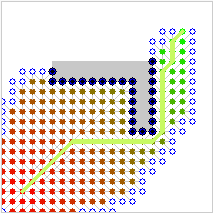
\includegraphics[width=0.28\textwidth]{pics/aStar.png}
  \end{center}
  \caption{Représentation d'une éxécution de A*\cite{wikiA*}}
\end{wrapfigure}
Cet algorithme possède quand même des limites. Il est effectivement efficace dans le cas où l'on considère les robots comme omniscient, connaissant l'environnement et, donc, connaissant la position de la source et des obstacles se trouvant dans l'environnement. Dans le cas de non-omniscience, l'arène est inconnue et on ne possède aucunes données à propos de celles-ci. Et c'est ici que se trouve le plus grand défaut de l'algorithme A*.

A* détermine un chemin complet de nœuds pour arriver d'un noeud départ à un noeud but. Lorsqu'il ne possède pas de données complètes à propos de l'arène, il est bloqué lors de son exécution et ne peut donc pas déterminer le chemin que doit suivre le robot. Il faudra adapter l'algorithme A* afin de remédier à ce problème.

\subsubsection{Algoritme de Dijkstra}
\cite{wikiDijkstra}

L’algorithme de Dijkstra est un algorithme servant à résoudre le problème du plus court chemin. Le principe de l'algorithme est le suivant:

Il s'agit de mettre en place progressivement un sous-graphe dans lequel sont classés les différents sommets. Un ordre croissant est établit entre les sommets et il est fixé en fonction de la distance minimale qui éloignent ces sommets à celui de départ. Cette distance correspond à la somme des nœuds parcourus.

Au début, les distances de chaque sommet par rapport au sommet de départ sont considérées comme infinie et on attribue à celui-ci une distance de 0.

Ensuite, au cours de chaque itération, les distances des sommets reliés par un nœud au dernier du sous-graphe sont mis à jour. Cette mis à jour consiste à ajouter la valeur du nœud à la distance séparant le sommet de départ à ce dernier sommet. Après cette mise à jour, l'ensemble des sommets, ne faisant pas partis du sous-graphe, sont examinés et celui qui possède la distance minimal y est ajouté.

Enfin, on répète l'exécution jusqu'à l'épuisement des sommets ou jusqu'à la sélection du sommet d'arrivée.
Voici 3 figures qui représentent un exemple du principe utilisé. Le but est de trouver le plus court chemin entre le point A et le point J. Comme dit précédemment, après chaque mise à jour, le sommet possédant la distance minimale est rajouté au sous graphe. La figure \ref{fig:dijkstra} représente bien cela.
\begin{figure}[h!]
        \centering
        \begin{subfigure}[h!]{0.4\textwidth}
                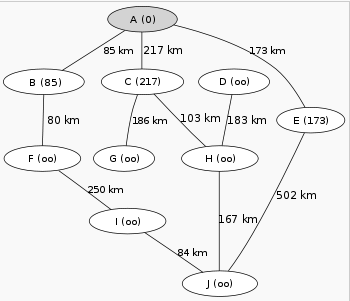
\includegraphics[width=\textwidth]{pics/dijk1.png}
                \caption{Mise à jour initiale\\\(\;\)}
        \end{subfigure}   \begin{subfigure}[h!]{0.4\textwidth}
                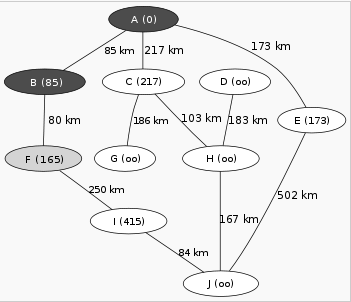
\includegraphics[width=\textwidth]{pics/dijk2.png}
                \caption{Mise à jour et construction du sous-graphe}
        \end{subfigure}

        \begin{subfigure}[h!]{0.4\textwidth}
                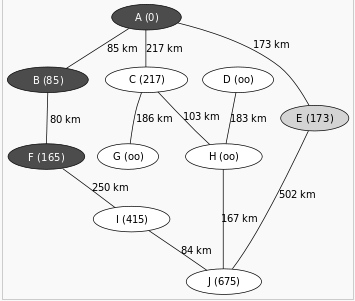
\includegraphics[width=\textwidth]{pics/dijk3.png}
                \caption{Mise à jour et graphe final}
        \end{subfigure}
        \caption{\label{fig:dijkstra}Représentation d'une éxécution de Dijkstra \cite{wikiDijkstra}}
\end{figure}


En effet, le sommet E est rajouté au sous graphe et non le sommet I car la distance à parcourir entre A et E est plus petite que entre A et I.

Il faut souligner que cet algorithme possède le même inconvénient qu'A*.

\begin{subappendices}
  \appsec{Implémentation du déplacement en Lua}
  \subsection{Evitement \emph{greedy}\label{app:implEvitGreedy}}
  \begin{lstlisting}[caption=Initialisation]
function init()
  robot.distance_scanner.enable()
  robot.distance_scanner.set_rpm(SCANNER_RPM)
  obstaclesTable={}
  for i=-PI+PI/DIR_NUMBER, PI-PI/DIR_NUMBER, 2*PI/DIR_NUMBER do
    obstaclesTable[i]=151
  end
  goalX=SOURCEX
  goalY=SOURCEY
end
  \end{lstlisting}
  \begin{lstlisting}[caption=Structure générale]
function step()
  odometry()
  obstaclesTable=updateObstaclesTable(obstaclesTable)
  move(goalX,goalY,obstaclesTable)
end
  \end{lstlisting}
  \begin{lstlisting}[caption=Rafraîchir la table des mesures à chaque pas, label=lst:updateObstaclesTable]
function updateObstaclesTable(tabl, which) 
  --tabl: the obstacleTable to refresh
  --(obstaclesTable or shortObstaclesTable)
  --which (string): which sensor to use
  --("short_range" or "long_range")
  local sensor, reading, angle, value, rAngle, rDistance
  for angle, value in pairs(tabl) do
    newValue=false
    for sensor, reading in pairs(robot
                                 .distance_scanner
                                 [which]) do
      rAngle = reading.angle
      rDistance=reading.distance
      if rDistance == -2 then rDistance=151 end
      if rDistance == -1 then rDistance=0 end
      if abs(angle-rAngle)<PI/DIR_NUMBER then
        if value>rDistance or not newValue then
          tabl[angle]=rDistance
          newValue = true
        end
      end
    end
  end
  return tabl
end
  \end{lstlisting}
  \begin{lstlisting}[caption=Fonction move]
function move(goalX,goalY,obstaclesTable)
  local goalDirection=findGoalDirection(posX,posY,goalX,goalY)
  local goalAngle=findGoalAngle(goalDirection, alpha)
  obstacleAvoidance(goalAngle, obstaclesTable)
end
  \end{lstlisting}
  \begin{lstlisting}[caption=Trouver la direction du goal vu du footbot]
function findGoalDirection(posX, posY, goalX, goalY)
  local deltaX=goalX-posX
  local deltaY=goalY-posY
  local goalDirection=math.atan(deltaY/deltaX)
  if deltaX<0 then
    goalDirection=goalDirection+PI
  end
  if goalDirection<0 then
    goalDirection=goalDirection+2*PI
  end
  return goalDirection
end

function findGoalAngle(goalDirection,alpha)
  local goalAngle=goalDirection-alpha
  if goalAngle>PI then
    goalAngle=goalAngle-2*PI
  end
  return goalAngle
end  
  \end{lstlisting}
  \begin{lstlisting}[caption=Trouver la direction optimale et la suivre]
function obstacleAvoidance(goalAngle, obstaclesTable)
  local bestAngle, bestDistance, angle, distance
  bestDistance = -1
  for angle, distance in pairs(obstaclesTable) do
    if distance>bestDistance
       or (distance==bestDistance and not bestAngle)
       or (distance==bestDistance
         and abs(angle-goalAngle)<abs(bestAngle-goalAngle)) then
      bestDistance = distance
      bestAngle = angle
    end
  end
  getToGoal(bestAngle, CONVERGENCE)
end
  \end{lstlisting}
  \begin{lstlisting}[caption=Fonction getToGoal]
function getToGoal(angle, conv)
   if angle>=0 then --goal is to the left
      vLeft=speed*((PI-angle)/PI)^conv
      vRight = 2*speed-vLeft
   else --goal is to the right
      vRight=speed*((PI+angle)/PI)^conv
      vLeft = 2*speed - vRight
   end
   robot.wheels.set_velocity(vLeft, vRight)
end
  \end{lstlisting}
  \subsection{Evitement d'obstacles proches \label{app:implEvitClose}}
  \begin{lstlisting}[caption=Capteur supplémentaire]
function step()
  ...
  emerProx, emerDir=readProxSensor()
  if emerProx>0 then
    emergencyAvoidance(emerProx, emerDir)
  else
  ...
end    
  \end{lstlisting}
  \begin{lstlisting}[caption=lecture du \emph{proximity sensor}]
function readProxSensor()
  local emerDir = 1
  local emerProx = robot.proximity[1].value
  for i=2,24 do
    if emerProx < robot.proximity[i].value
       or (emerProx == robot.proximity[i].value
           and abs(12-emerDir)<abs(12-i)) then
      emerDir = i
      emerProx = robot.proximity[i].value
    end
  end
  return emerProx, emerDir
end
  \end{lstlisting}

  \begin{lstlisting}[caption=Fonction emergencyAvoidance]
function emergencyAvoidance(emerProx,emerDir)
  local vLeft, vRight
  if emerDir <= 12 then --Obstacle is to the left
    vRight=((1-emerProx)^EMER_PROX_DEP*emerDir
             -EMER_DIR_DEP)
           *speed/11
    vLeft=2*speed-vRight
  else --Obstacle is to the right
    vLeft=((1-emerProx)^EMER_PROX_DEP*(25-emerDir)
            -EMER_DIR_DEP)
          *speed/11
    vRight=2*speed-vLeft
  end
  robot.wheels.set_velocity(vLeft, vRight)
end    
  \end{lstlisting}

  \appsec{Ajout d'une composante aléatoire à l'évitement}

\end{subappendices}
